5.	En el panel de controles de todo osciloscopio, suele haber un punto de prueba (TP) donde hay disponible una señal, generada internamente, de 1KHz, con forma de onda cuadrada que según lo indicado habitualmente en los manuales se emplea para “calibra la punta de pruebas”. Dicho procedimiento se realiza:
\begin{enumerate}
\item[A.] Con la punta en posición X10 y es para calibrar la base de tiempos.
\item[B.] Con la punta en posición X10 y es para compensar la respuesta en frecuencia.
\item[C.] Con la punta en la posición X1 y es para compensar la respuesta en frecuencia.
\item[D.] Con la punta en la posición X1 y es para calibrar el nivel de disparo.
\end{enumerate}

\vspace{1em}

6.	La calibración de la punta, se hace observando la forma de onda cuadrada, y normalmente debe retocarse un ajuste que suele encontrarse:
\begin{enumerate}
\item[A.] En el panel del instrumento y se accede mediante un destornillador de plástico.
\item[B.] En la propia punta de pruebas, y se accede mediante un destornillador de plástico.
\item[C.] En la propia punta de pruebas, y para ello suele haber una llave de tres posiciones.
\item[D.] Debe retirarse la cubierta del osciloscopio ya que el ajuste suele estar en su interior.
\end{enumerate}
\vspace{1em}
7.	Por lo general todos los osciloscopios de doble trazo disponen, en el selector de “Modo Vertical”, de una posición denominada “ADD” (Suma). Este modo suele utilizarse juntamente con la opción “INV” (inversión) de uno de los canales Y. Cuando un osciloscopio se emplea de esta forma:
\begin{enumerate}
\item[A.] Es posible determinar la diferencia de fase entre dos señales de la misma frecuencia.
\item[B.] Funciona como un instrumento de canal único y entrada diferencial.
\item[C.] Permite visualizar una señal restando la componente de CC.
\item[D.] No es un modo que tenga utilidad. Debe ser evitado.
\end{enumerate}

\vspace{1em}

8.	La siguiente imagen representa un oscilograma obtenido con un osciloscopio, cuyos controles se encuentra en las siguientes posiciones: 
A.	Eje Y= 2V/div;
B.	Base de T = 1ms/div. 
C.	La sonda de pruebas se encuentra en la posición X 10, 
D.	La forma de onda observada no tiene componente de CC.
 
\begin{figure}[H]
    \centering
	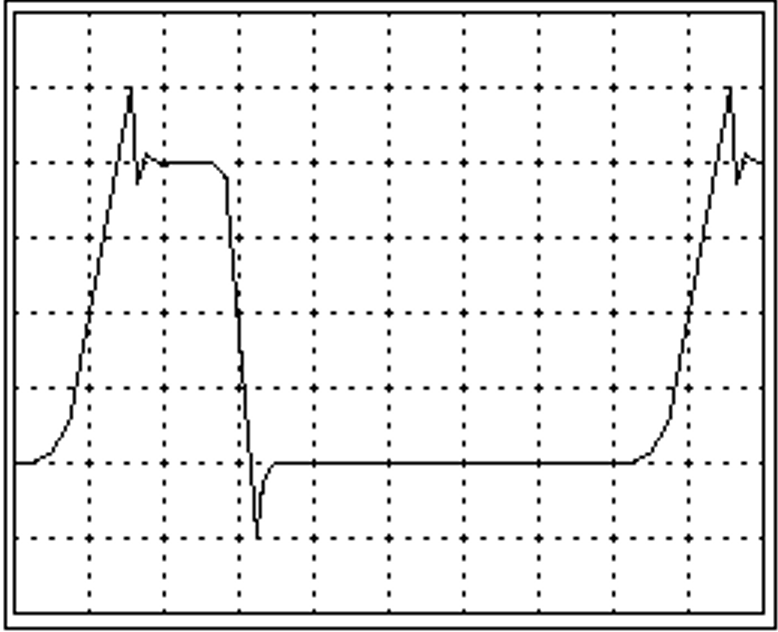
\includegraphics[width=0.4\textwidth]{images/conclusiones.png}
	\caption{Señal en x10 con acoplamiento en CA}
	\label{fig:calibracion}
\end{figure} 

E.	Se pide determinar:
\begin{enumerate}
\item[1.] El ciclo de trabajo de la forma de onda observada.
\item[2.] El valor eficaz de la tensión.
\end{enumerate}